\documentclass[../thesis.tex]{subfiles}
\begin{document}

\chapter{Simulation model}
\label{chp:model}

Within this part the creation process of the simulation model will be explained in greater detail. At first the three basic equations the software solves will be given followed by a brief overview of the steps taken to create the model. Then the model's results are explained and compared to already done experiments for validation.

\section{model setup}
\label{sec:mod_setup}

In this section the steps needed to create the model within \texttt{ANSYS FLUENT} are explained.

\subsection{geometry creation}
The first of the model creation in \texttt{ANSYS FLUENT} is the modeling of the system's geometry. This geometry can either be created using the tools \texttt{ANSYS FLUENT} provides it self or be imported from an already existing CAD model. Within this work the geometry is created using ANSYS DesignModeler. In \autoref{fig:ansys_geometry} the designed model is shown and the used dimensions are listed in \autoref{tab:ansys_design}.

\begin{figure}[htbp]
	\centering
	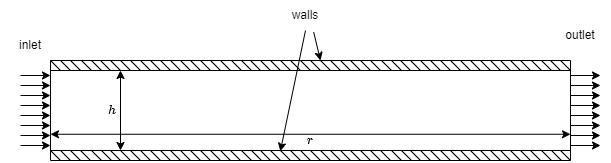
\includegraphics[width=\textwidth]{geometry}
	\caption{model geometry}
	\label{fig:ansys_geometry}
\end{figure}

\begin{table} [htb]
	\centering
	\caption{example model geometry dimensions}
	\begin{tabular}{ ccc }
		\hline
		variable & value & unit \\
		\hline
		$r$ & 30.0 & mm \\
		$h$ & 0.6 & mm \\
		\hline
		\label{tab:ansys_design}
	\end{tabular}
\end{table}

$h$ represents the height of the Hele-Shaw cell and $r$ is the radius of the cell. A value of 30mm is chosen here to reduce the amount of computational effort instead of modeling the hole cell with it's 50mm radius.

\subsection{meshing}

The next step in model design following the procedure shown in \autoref{fig:cdf_procedure} in \autoref{chp:theory} is meshing. An example of the generated mesh can be seen in \autoref{fig:ansys_meshing}.
\begin{figure}[htb]
	\centering
	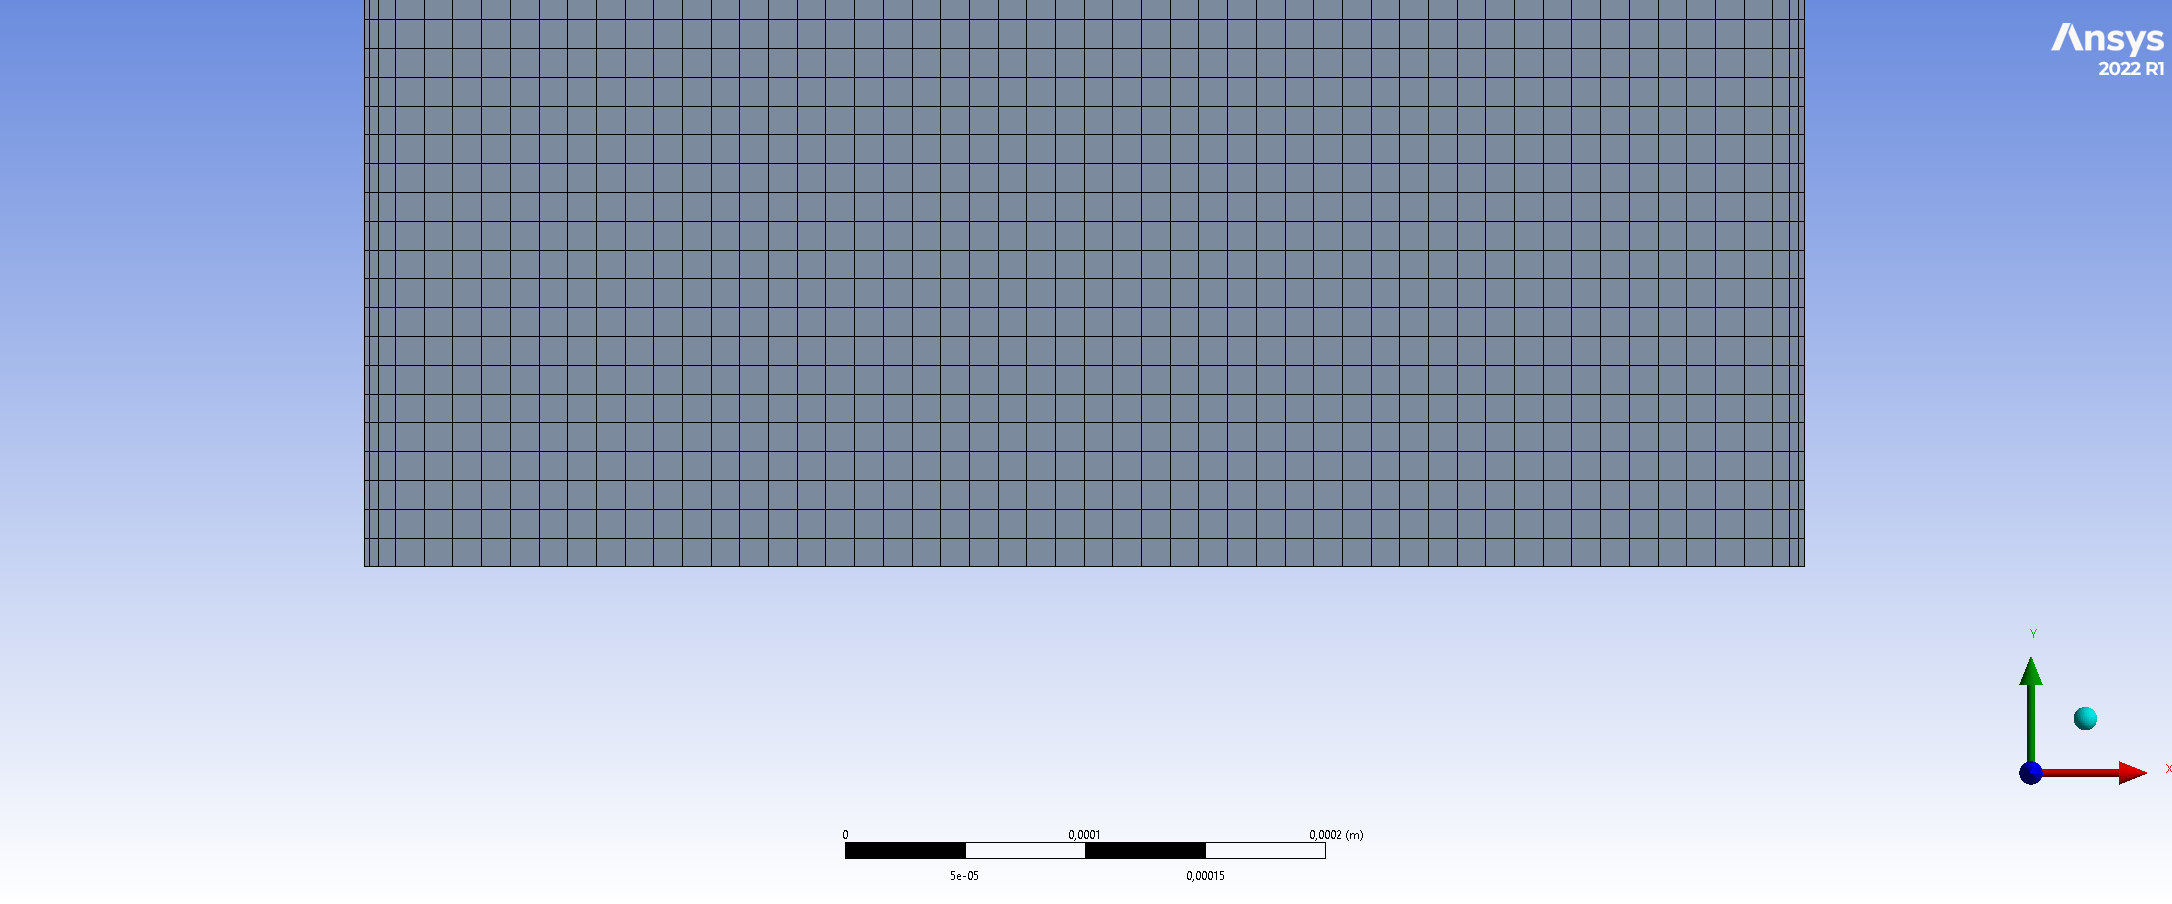
\includegraphics[scale=0.25]{Mesh}
	\caption{Ansys Meshing example}
	\label{fig:ansys_meshing}
\end{figure}
The figure shows the reactor's inlet section. The goal in meshing was to create rectangular grid out of squares or rectangles. Near the walls, that begin on the left and right side of the inlet, the mesh resolution is increased using two inflation layers. That is done to resolve the boundary layer of the flow near the walls. Having a mesh consisting mostly out of squares and rectangles is advantageous because the algorithm only stores the values at the cell's centre as mentioned in \autoref{sec:QUICK}. Having a mesh that can be seen as a 2 dimensional array makes post-processing a lot easier. How the results are extracted from the model's output will be explained in \autoref{sec: model res} in greater detail.

\subsection{solver settings}
\label{sec: setup}

To setup the model at first a few basic configuration steps need to done. The Settings that need to be applied are listed in \autoref{tab:ansys_setup_general}.

\begin{table} [htb]
	\centering
	\caption{General settings}
	\begin{tabular}{ ccc }
		\hline
		Section & Setting & value \\
		\hline
		Solver & Type & Pressure-Based \\
		Solver & Velocity Formulation & Absolute  \\
		Solver & Time &  Transient  \\
		Solver & 2D Space & Axisymmetric \\
		\hline
		\label{tab:ansys_setup_general}
	\end{tabular}
\end{table}
The type of solver chosen is a Pressure-Based and is left as the default value. The velocity formulation is set to \texttt{Absolute} because the input velocity is set to an absolute value and all exported velocity values should be absolute as well. The \texttt{Time} setting is set to \texttt{Transient} because the flow modelled is not stationary and the interest is in results during the hole model simulation run. The \texttt{2D Space} settings has a value of \texttt{Axisymmetric} due to the axisymmetric nature of the model. 

With these general settings done the used models need to be activated. The used models settings are given in \autoref{tab:ansys_setup_models}. The Viscous model is set to \texttt{Laminar} because laminar flow conditions are used for the simulation. Because a reaction is part of the model the energy variable needs to be set to \texttt{On}.

\begin{table} [htb]
	\centering
	\caption{model settings}
	\begin{tabular}{ cc }
		\hline
		variable & value \\
		\hline
		Energy & On \\
		Viscous & Laminar \\
		Species & (Species Transport, Reactions)  \\
		\hline
		\label{tab:ansys_setup_models}
	\end{tabular}
\end{table}

After the correct models are turned on and parametrized the species taking part within the model are defined. Within this case 4 fluids are needed. The example configuration of one of the fluids taking part within the reaction is shown in \autoref{tab:ansys_setup_materials}. The table shows the configuration of one of the educts.
\begin{table} [htb]
	\centering
	\caption{Example fluid settings}
	\begin{tabular}{ ccc }
		\hline
		variable & value & unit \\
		\hline
		\\[-1em]
		$\rho$ & 1000 & $\frac{\text{kg}}{\text{m³}}$ \\
		\\[-1em]
		$\nu$ & 0.001003 & $\frac{\text{m²}}{s}$ \\
		\\[-1em]
		$M$ & 100 & $\frac{\text{g}}{\text{mol}}$ \\
		\\[-1em]
		$D$ & 8.22e-10 & $\frac{\text{m²}}{s}$\\
		\\[-1em]
		\hline
		\label{tab:ansys_setup_materials}
	\end{tabular}
\end{table}
All other values, namely enthalpies and other thermodynamic properties are the same for all the fluids and equal to the values of water. Since 3 fluids take part in the reaction and 4 fluids are needed to setup the model the yet missing fluid is water. It is needed to be able to set a molar concentration at the inlet that is lower than the maximum of 1. After this the values from the fluids should be carried over to the mixture configuration within the new existing Mixture tab. With the mixture settings the reaction parameters are set. The parameters set for the reaction are stated in \autoref{tab:ansys_setup_rection}.
\begin{table} [htb]
	\centering
	\caption{reaction settings}
	\begin{tabular}{ ccc }
		\hline
		variable & value & unit \\
		\hline
		Reaction Type & Volumetric & - \\
		Stoich. Coefficient fluid\_a & 1 & - \\
		Stoich. Coefficient fluid\_b & 1 & - \\
		Stoich. Coefficient fluid\_c & 1 & - \\
		Rate Exponent fluid\_a & 1 & - \\
		Rate Exponent fluid\_b & 1 & - \\
		Rate Exponent fluid\_c & 0 & - \\
		Pre-Exponential Factor & 1e15 & - \\
		\\[-1em]
		Activation Energy & 1e4 & $\frac{\text{J}}{\text{mol}}$ \\
		\\[-1em]
		\hline
		\label{tab:ansys_setup_rection}
	\end{tabular}
\end{table}
To achieve a nearly instant reaction when molecules of the two species A and B meet the rate constant which also known as Pre-Exponential Factor (see \autoref{eqn:reaction}) is set to a very high value. The Activation Energy is set to a value that the given temperature is high enough to let the reaction happen.

After the reaction is setup correctly the boundary conditions are being set. Conditions need to be set for the inlet, outlet and the walls. All information needed to configure the boundary conditions are visible in \autoref{tab:ansys_setup_boundary}

\begin{table} [htb]
	\centering
	\caption{boundary conditions}
	\begin{tabular}{ cccc }
		\hline
		place & variable & value & unit \\
		\hline
		inlet & Type & velocity-inlet & - \\
		inlet & Velocity Specification Method & Magnitude, Normal to Boundary & - \\
		\\[-1em]
		inlet & Velocity Magnitude & e.g. 4e-3 & $\frac{\text{m}}{\text{s}}$ \\
		\\[-1em]
		inlet & Temperature & 300 & K \\
		inlet & fluid\_a & 5.4e-4 & - \\
		outlet & Type & pressure-outlet & - \\
		outlet & Gauge Pressure & 20 & Pa \\
		outlet & Prevent Reverse Flow & yes & - \\
		wall & Type & wall & - \\
		wall & Wall Motion & Stationary Wall & - \\
		wall & Shear Condition & No Slip & - \\
		\hline
		\label{tab:ansys_setup_boundary}
	\end{tabular}
\end{table}
There is a homogenous velocity profile set at the inlet normal to the boundary. At the inlet the amount of $fluid\_a$ has to set as a mole fraction as well. To get matching conditions to the already performed experiments the mole fraction needs to be calculated from a given concentration. Assuming the values from \autoref{tab:ansys_setup_molefrac} are known the mole fraction can be calculated using \autoref{eqn:molefrac}.

\begin{table} [htb]
	\centering
	\caption{needed variables for mole and mass fraction calculation}
	\begin{tabular}{ cccc }
		\hline
		variable & description & value & unit \\
		\hline
		\\[-1em]
		$M_{water}$ & Molar Mass water & 18 & $\frac{\mathrm{g}}{\mathrm{mol}}$ \\
		\\[-1em]
		$M_{fluid\_a}$ & Molar Mass $fluid\_a$ & 100 & $\frac{\mathrm{g}}{\mathrm{mol}}$ \\
		\\[-1em]
		$M_{fluid\_b}$ & Molar Mass $fluid\_b$ & 100 & $\frac{\mathrm{g}}{\mathrm{mol}}$ \\
		\\[-1em]
		$\rho_{water}$ & Density water & 1000 & $\frac{\mathrm{kg}}{\mathrm{m}^3}$ \\
		\\[-1em]
		$c_{fluid\_a}$ & Concentration $fluid\_b$ & 0.03 & $\frac{\mathrm{mol}}{\mathrm{l}}$ \\
		\\[-1em]
		$c_{fluid\_b}$ & Concentration $fluid\_b$ & 0.03 & $\frac{\mathrm{mol}}{\mathrm{l}}$ \\
		\\[-1em]
		$c_{water}$ & Concentration water & 55.55 & $\frac{\mathrm{mol}}{\mathrm{l}}$ \\
		\\[-1em]
		$Q$ & inlet flow rate &  e.g. 0.144 & $\frac{\mathrm{ml}}{\mathrm{min}}$ \\
		\\[-1em]
		\hline
		\label{tab:ansys_setup_molefrac}
	\end{tabular}
\end{table}

\begin{equation}
	\label{eqn:molefrac}
	x_{B} =\dfrac{\dot{n_{B}}}{\dot{n_{B}} + \dot{n_{W}}} = \dfrac{c_{B} \cdot Q}{c_{B} \cdot Q + c_{W} \cdot Q} = \dfrac{c_{B}}{c_{B} + c_{W}} \approx 0 \text{.}00054
\end{equation}
Since the concentration for $fluid\_{a}$ within the internal domain has to be setup as mass fraction the needed value can be calculated using \autoref{eqn:massfrac}.

\begin{equation}
	\label{eqn:massfrac}
	\varphi_{A} =\dfrac{n_{A} \cdot M_{A}}{n_{A} \cdot M_{A} + n_{W} \cdot M_{W}} = \dfrac{c_{A} \cdot M_{A}}{c_{A} \cdot M_{A} + c_{W} \cdot M_{W}} \approx \text{0.003}
\end{equation}

The temperature is set to 300 K at the inlet and within the hole internal domain. The outlet is configured to be a pressure outlet without reverse flow to get physical valid results. At the walls the usual conditions applied to walls are set with no slip and stationary.

The next step performed is to setup the solution methods as shown in \autoref{tab:ansys_setup_sol_methods}. As the solving scheme the PISO algorithm is used, that is explained in \autoref{sec:sol_method}. For spatial discretization second order methods, as explained in \autoref{sec:QUICK}, are used. 
\begin{table} [htb]
	\centering
	\caption{solution methods}
	\begin{tabular}{ ccc }
		\hline
		tab & setting & method \\
		\hline
		Pressure-Velocity Coupling & Scheme & PISO \\
		Spatial Discretization & Pressure & Second Order \\
		Spatial Discretization & Momentum & QUICK \\
		Spatial Discretization & $fluid\_a$ & Second Order Upwind \\
		Spatial Discretization & $fluid\_b$ & Second Order Upwind \\
		Spatial Discretization & $fluid\_c$ & Second Order Upwind \\
		Spatial Discretization & Energy & Second Order Upwind \\
		\hline		
		\label{tab:ansys_setup_sol_methods}
	\end{tabular}
\end{table}

As a last step in the model creation procedure the time settings need to be set. An adaptive method is chosen which is based on the CFL-Number $c$. The CFL-Number is another name for the Courant-Number. It is best practice to keep this number below or equal to 1 for stability reasons. This can be otherwise thought of as a limiting factor in a way that to rapid changes from one cell to the next one between time steps are inhibited.
  
In this model the Courant-Number is set to 1 and the initial time step size is set to 0.01 seconds to get a compromise between simulation stability and calculation time. The time step size is updated after every calculation. The factor for time step changes are limited to 0.5 on the lower and 2 at the upper end. The time step algorithm decides for a time step change based on the Courant-Number. In most cases the time step used by the solver has a value close to the minimum time step size of 0.001 seconds. 

In addition to the model's time settings the interval the results are exported at need to be set. This in addition to the exported variables of interest can be set under $\texttt{Solution} \rightarrow \texttt{Activities} \rightarrow \texttt{Manage...}$.

\begin{table} [htb]
	\centering
	\caption{time settings}
	\begin{tabular}{ ccc }
		\hline
		variable & value & unit \\
		\hline
		Type & Adaptive & - \\
		Method & CFL-Based & - \\
		Duration Specification Method & Total Time & -\\
		Total Time & e.g. 20 & s \\
		Courant Number & 1 & - \\
		Fixed Timsteps & 1 & - \\
		Initial Time Step Size & 0.01 & s \\
		Max Iteration/Time Step & 30 & - \\
		Time Step Size Update Interval & 1 & - \\
		Minimum Time Step Size & e.g. 0.001 & s \\
		Maximum Time Step Size & e.g. 0.5 & s \\
		Minimum Step Change Factor & 0.5 & - \\
		Maximum Step Change Factor & 2 & - \\		
		\hline
		\label{tab:ansys_setup_time}
	\end{tabular}
\end{table}

\section{model evolution}
\label{sec: mod_evol}

Here the steps taken to receive the final model for each case are explained.

\subsection{mesh dependency}

To achieve good results from a CFD-model the solution obtain should be independent of the grid element size. 
Do do that for each case different meshes with different grid densities are created as shown in \autoref{tab: reactor meshes}.

\begin{table} [htb]
	\centering
	\caption{case meshes}
	\begin{tabular}{ ccc }
		\hline
		reactor height [mm] & element size [m] & mesh elements \\
		\hline
		0.2 & 6e-6 & 185000\\
		0.2 & 4e-6 & 405000\\
		0.2 & 2e-6 & 1560000\\
		0.4 & 12e-6 & 92500\\
		0.4 & 8e-6 & 202500\\
		0.4 & 4e-6 & 780000\\
		0.6 & 4e-6 & 1155154\\
		0.6 & 2e-6 & 4560304\\
		\hline		
		\label{tab: reactor meshes}
	\end{tabular}
\end{table}

Each case is run for the coarsest mesh and the results are inspected. The first indication for grid independent results can be extracted from the Courant-Number field. An example of a right and wrong field is shown in \autoref{fig: good_courant}. If as within the example, the field shows values higher than 1 the next finer mesh is chosen and the simulation is run again. If that is not the case the grid is chosen and the run is called successful.

\begin{figure}[htb]
	\centering
	\subfloat[\centering Wrong Courant-Number field for an example case]{{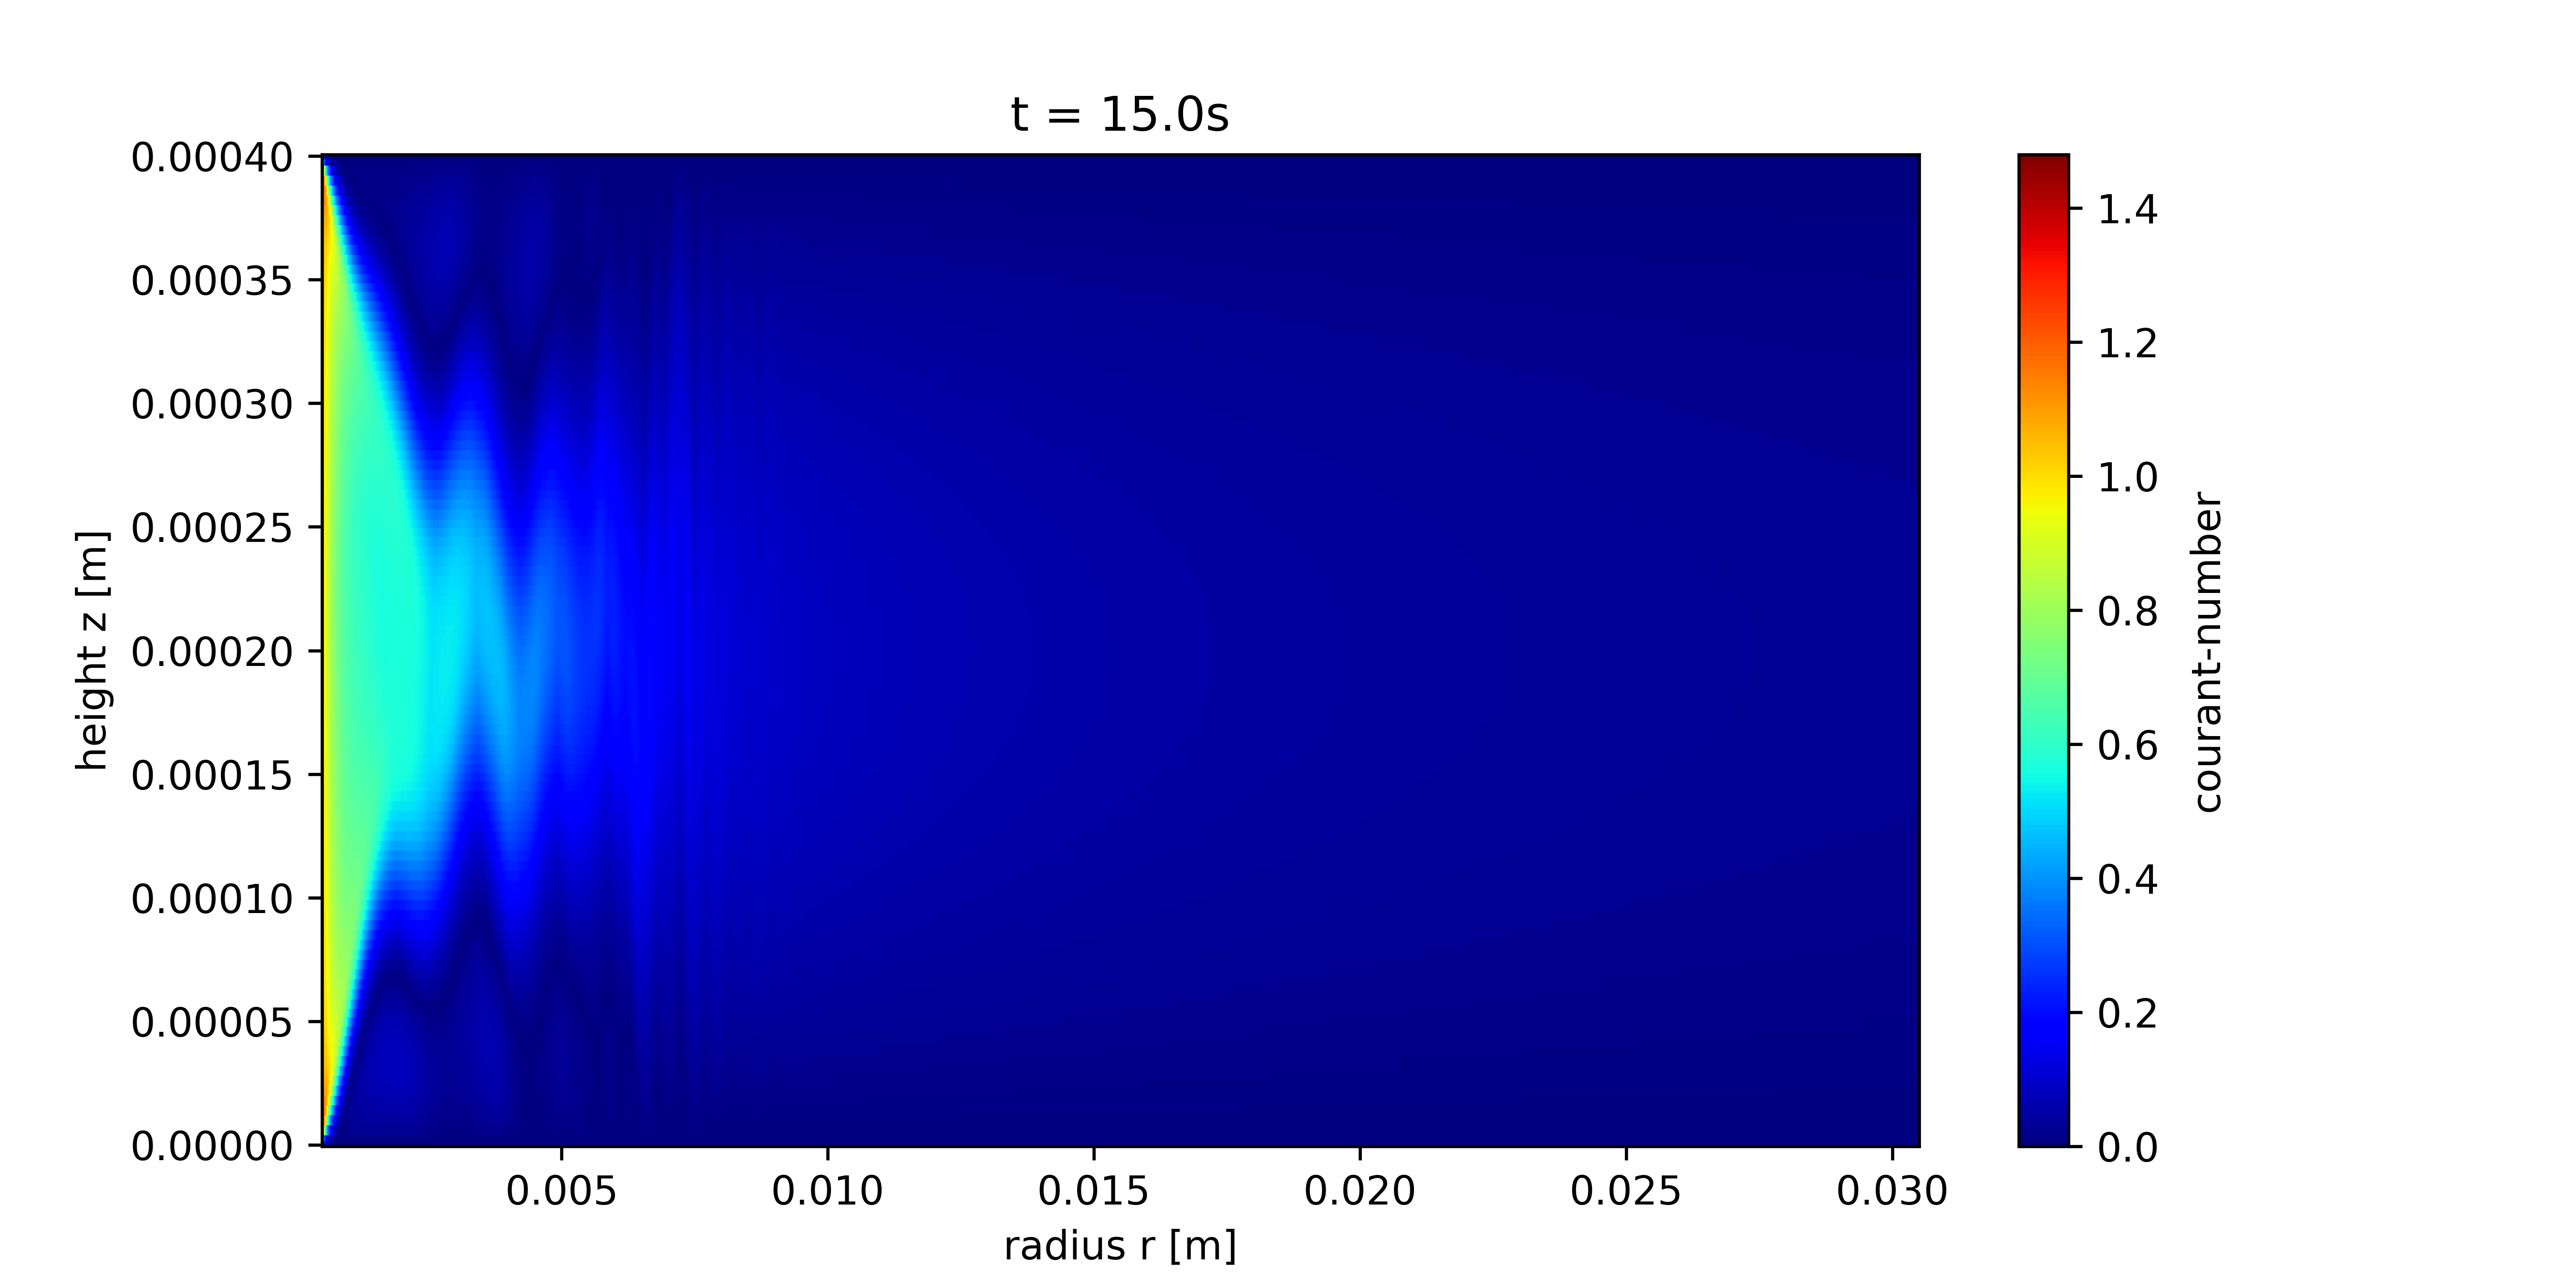
\includegraphics[scale=0.7]{bad_courant} }}
	\qquad
	\subfloat[\centering Right Courant-Number field for another example case]{{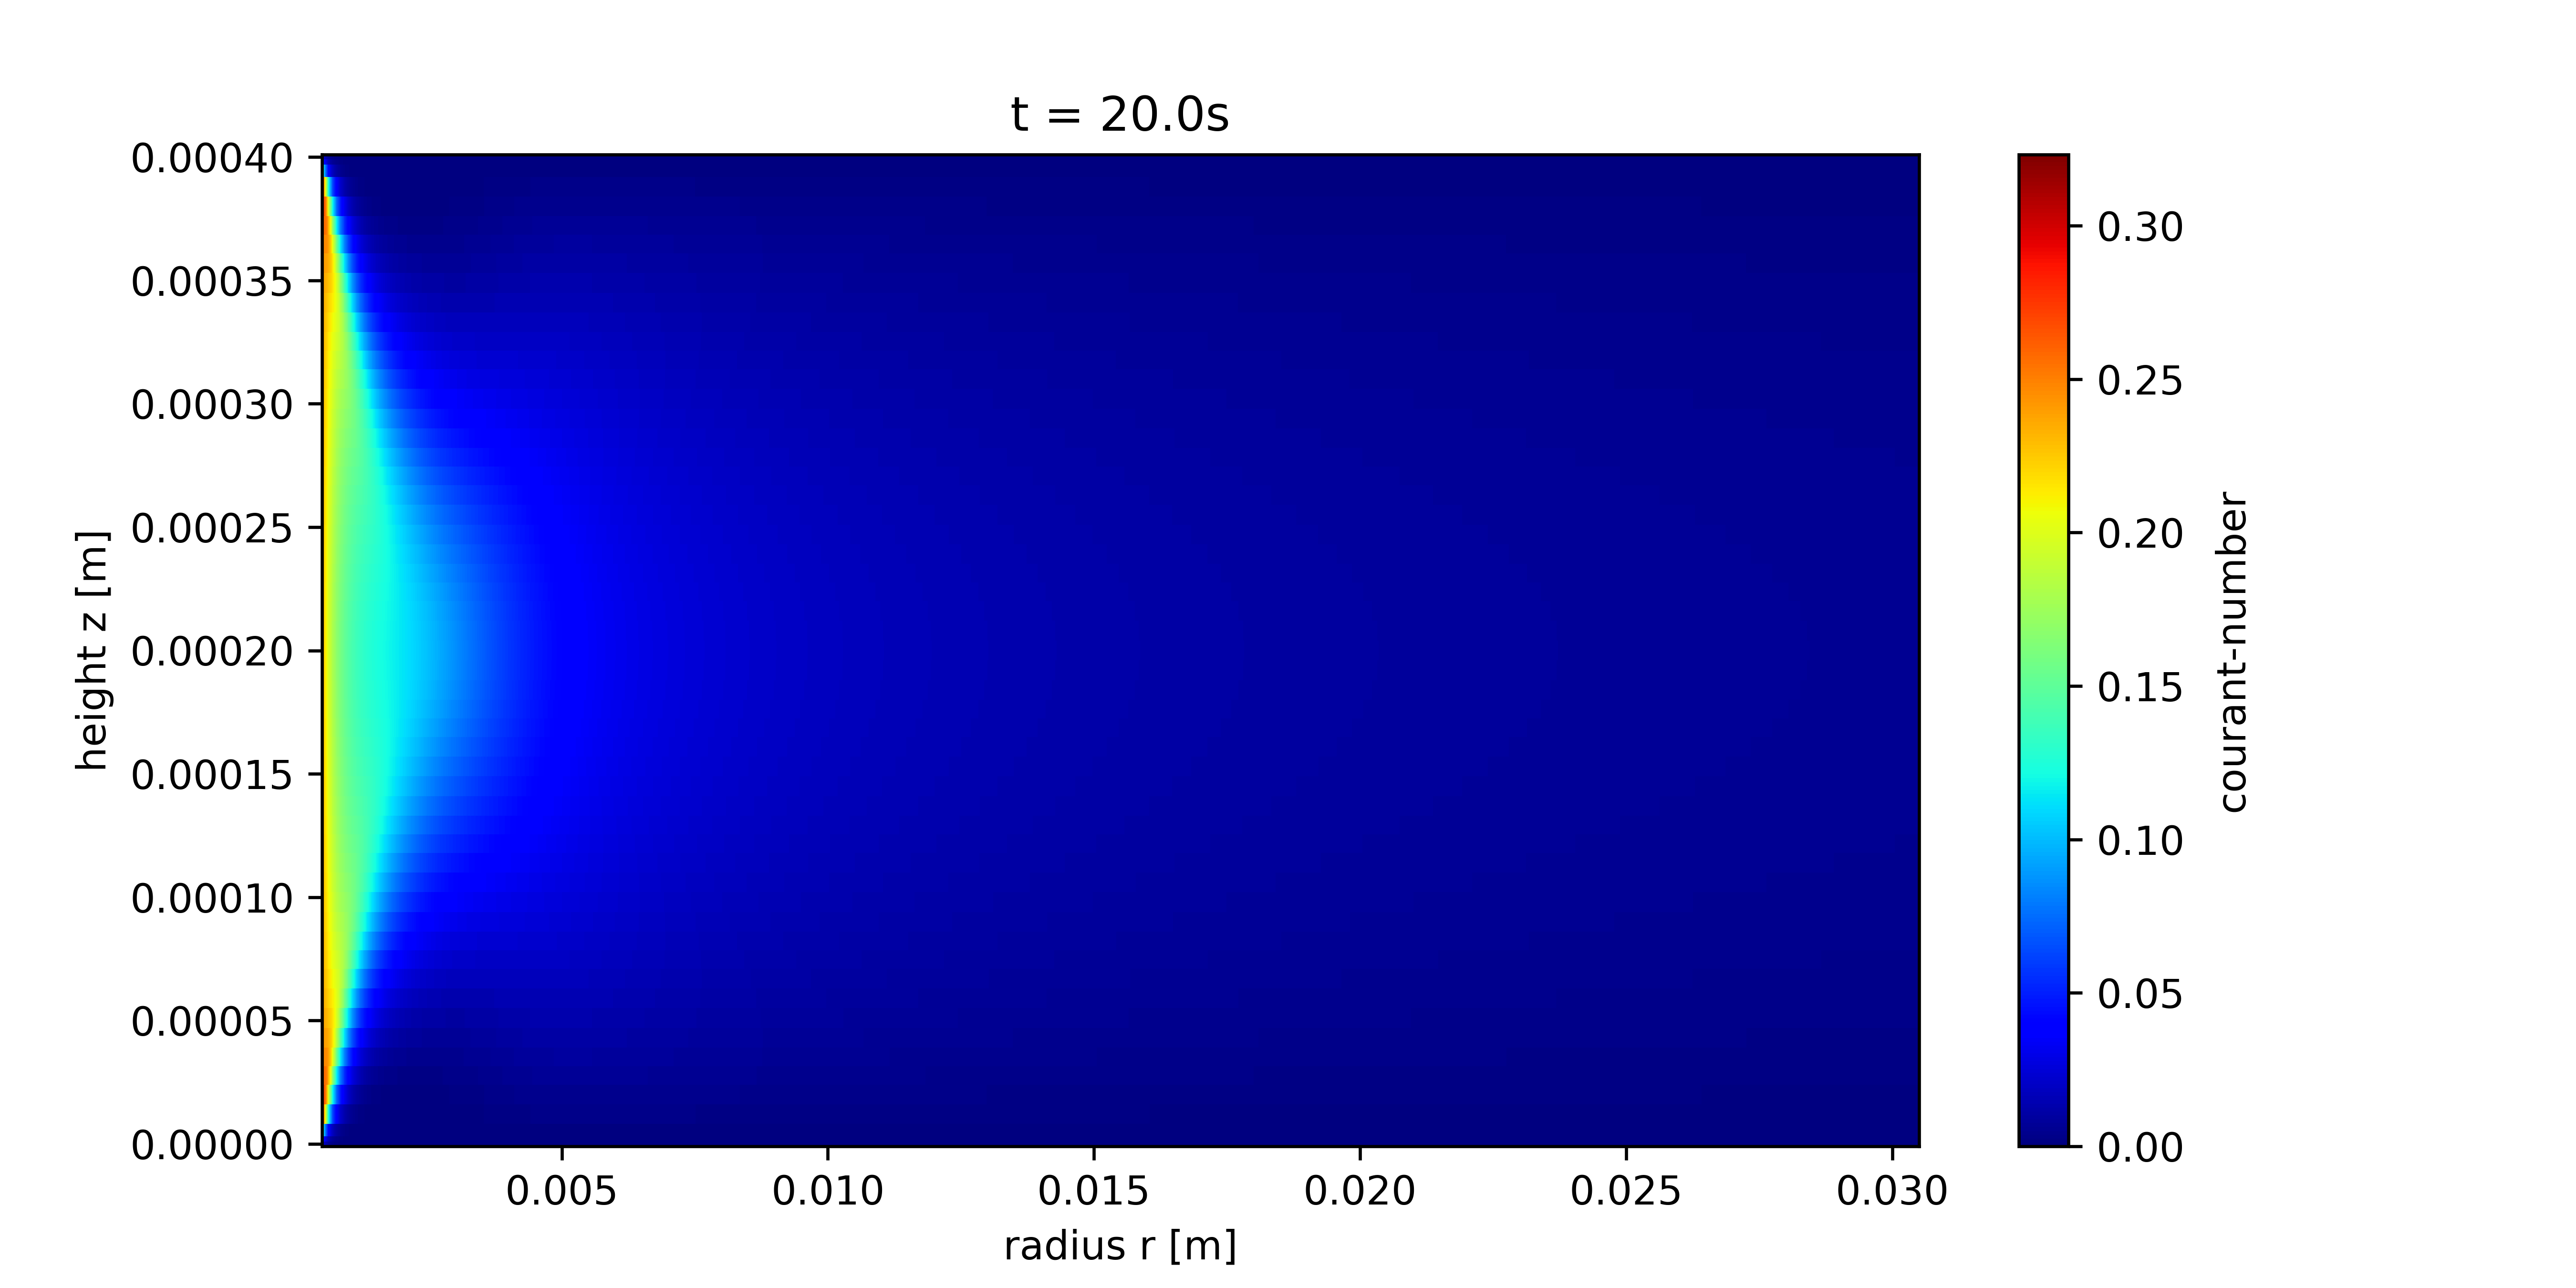
\includegraphics[scale=0.7]{good_courant} }}
	\caption{wrong and right example of Courant-Number field for mesh dependency study}
	\label{fig: good_courant}
\end{figure}

With this method a fine enough mesh for each case is chosen so that the results can be trusted. It's not the optimal mesh grid size but the approach provides a mesh that produces believable results for a given case.

\subsection{Cases Setup}

For the Peclet-Number 3 different values are chosen and for the Schmidt number 2 values are implemented. These values are in case of $Pe$ 500, 931 and 2050. The Schmidt number $Sc$ has either a value of 2430 or 12000. The Schmidt number mostly influences the diffusion coefficient as the viscosity $\nu$ does not change a lot between the two chosen values. Having fixed the Schmidt number and the diffusion coefficient, the Peclet-Number mostly influences the input velocity. An overview of the performed cases and their input variable values can be seen in \autoref{tab: cases}. Besides the reactor height $h$, the Peclet-Number $Pe$ and other needed input variables, the simulation time and export time in seconds need to be set. The simulation time is the physical time that represents for how long the model should be simulated. The export time sets the time interval in seconds at which results are exported during the transient simulation. These results, that contain all the values for all variables of interest for each cell, are the basis for further analysis. How the results are obtained and how they are further processed is explained in \autoref{sec: model res}.

\begin{landscape}
	\begin{table}[htb]
		\centering
		\caption{simulation cases}
		\label{tab: cases}
		\small
		\begin{tabular}{cccccccccc}
			\textbf{h [m]} & \textbf{Pe} & \textbf{Sc} & \textbf{$\nu$ [m²/s]} & \textbf{$D$ [m²/s]} & \textbf{u [m/s]} & \textbf{$x_A$} & \textbf{$\varphi_B$} & \textbf{simulation time [s]} & \textbf{export time [s]} \\
			\hline
			2.00E-04            & 500         & 2430        & 1.00E-06               & 4.11E-10               & 1.03E-03              & 5.40E-04      & 3.00E-03        & 60                            & 0.5                       \\
			2.00E-04            & 500         & 12000       & 1.20E-06               & 1.00E-10               & 2.50E-04              & 5.40E-04      & 3.00E-03        & 60                            & 0.1                       \\
			2.00E-04            & 500         & 120000      & 1.20E-06               & 1.00E-11               & 2.50E-05              & 5.40E-04      & 3.00E-03        & 60                            & 0.1                       \\
			2.00E-04            & 931         & 2430        & 1.00E-06               & 4.11E-10               & 1.91E-03              & 5.40E-04      & 3.00E-03        & 60                            & 0.5                       \\
			2.00E-04            & 931         & 12000       & 1.20E-06               & 1.00E-10               & 4.66E-04              & 5.40E-04      & 3.00E-03        & 60                            & 0.1                       \\
			2.00E-04            & 931         & 120000      & 1.20E-06               & 1.00E-11               & 4.66E-05              & 5.40E-04      & 3.00E-03        & 60                            & 0.1                       \\
			2.00E-04            & 2050        & 2430        & 1.00E-06               & 4.11E-10               & 4.21E-03              & 5.40E-04      & 3.00E-03        & 60                            & 0.5                       \\
			2.00E-04            & 2050        & 12000       & 1.20E-06               & 1.00E-10               & 1.02E-03              & 5.40E-04      & 3.00E-03        & 60                            & 0.1                       \\
			2.00E-04            & 2050        & 120000      & 1.20E-06               & 1.00E-11               & 1.02E-04              & 5.40E-04      & 3.00E-03        & 60                            & 0.1                       \\
			4.00E-04            & 500         & 2430        & 1.00E-06               & 4.11E-10               & 5.14E-04              & 5.40E-04      & 3.00E-03        & 60                            & 0.5                       \\
			4.00E-04            & 500         & 12000       & 1.20E-06               & 1.00E-10               & 1.25E-04              & 5.40E-04      & 3.00E-03        & 60                            & 0.1                       \\
			4.00E-04            & 500         & 120000      & 1.20E-06               & 1.00E-11               & 1.25E-05              & 5.40E-04      & 3.00E-03        & 60                            & 0.1                       \\
			4.00E-04            & 931         & 12000       & 1.20E-06               & 1.00E-10               & 2.33E-04              & 5.40E-04      & 3.00E-03        & 60                            & 0.1                       \\
			4.00E-04            & 931         & 2430        & 1.00E-06               & 4.11E-10               & 9.57E-04              & 5.40E-04      & 3.00E-03        & 60                            & 0.5                       \\
			4.00E-04            & 931         & 120000      & 1.20E-06               & 1.00E-11               & 2.33E-05              & 5.40E-04      & 3.00E-03        & 60                            & 0.1                       \\
			4.00E-04            & 2050        & 12000       & 1.20E-06               & 1.00E-10               & 5.12E-04              & 5.40E-04      & 3.00E-03        & 60                            & 0.5                       \\
			4.00E-04            & 2050        & 2430        & 1.00E-06               & 4.11E-10               & 2.10E-03              & 5.40E-04      & 3.00E-03        & 60                            & 0.5                       \\
			4.00E-04            & 2050        & 120000      & 1.20E-06               & 1.00E-11               & 5.12E-05              & 5.40E-04      & 3.00E-03        & 60                            & 0.1                       \\
			6.00E-04            & 500         & 2430        & 1.00E-06               & 4.11E-10               & 3.43E-04              & 5.40E-04      & 3.00E-03        & 60                            & 0.5                       \\
			6.00E-04            & 500         & 12000       & 1.20E-06               & 1.00E-10               & 8.33E-05              & 5.40E-04      & 3.00E-03        & 60                            & 0.5                       \\
			6.00E-04            & 500         & 120000      & 1.20E-06               & 1.00E-11               & 8.33E-06              & 5.40E-04      & 3.00E-03        & 60                            & 0.5                       \\
			6.00E-04            & 931         & 12000       & 1.20E-06               & 1.00E-10               & 1.55E-04              & 5.40E-04      & 3.00E-03        & 60                            & 0.5                       \\
			6.00E-04            & 931         & 2430        & 1.00E-06               & 4.11E-10               & 6.38E-04              & 5.40E-04      & 3.00E-03        & 60                            & 0.5                       \\
			6.00E-04            & 931         & 120000      & 1.20E-06               & 1.00E-11               & 1.55E-05              & 5.40E-04      & 3.00E-03        & 60                            & 0.5                       \\
			6.00E-04            & 2050        & 12000       & 1.20E-06               & 1.00E-10               & 3.41E-05              & 5.40E-04      & 3.00E-03        & 60                            & 0.5                       \\
			6.00E-04            & 2050        & 2430        & 1.00E-06               & 4.11E-10               & 1.40E-03              & 5.40E-04      & 3.00E-03        & 60                            & 0.5                       \\
			6.00E-04            & 2050        & 120000      & 1.20E-06               & 1.00E-11               & 3.41E-05              & 5.40E-04      & 3.00E-03        & 60                            & 0.5						\\
			\hline      
		\end{tabular}
	\end{table}
\end{landscape}

\section{validation}
\label{chp:validation}

Within this chapter the model validation is explained and described. At first the experimental setup used in the performed experiments is shown and then the experimental and model results are explained. After that a comparison is done to show that the model is performing as expected.

\subsection{experimental setup and results}

The experiments used for validating the developed model where done using a sounding rocket as part of the \texttt{MORABA} (\textbf{Mo}bile \textbf{Ra}cketen \textbf{Ba}sis) \cite{stamminger2012moraba} setup. The mission's name was \texttt{TEXUS-57}. The experimental setup as shown in \cite{stergiou2022effects} is visible in \autoref{fig: experiment}.
\begin{figure}[htbp]
	\centering
	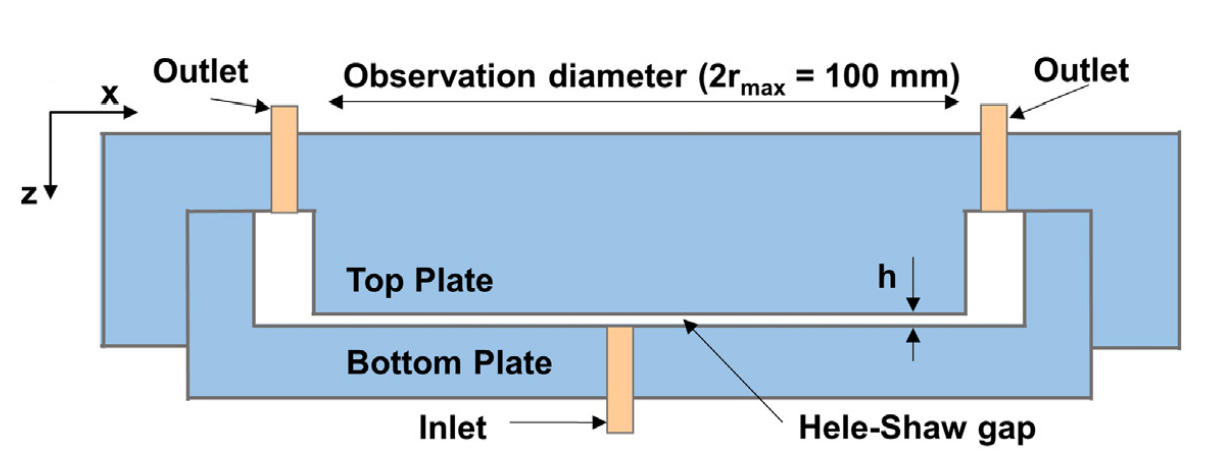
\includegraphics[scale=0.4]{experimental_setup}
	\caption{experimental setup for validation \cite{stergiou2022effects}}
	\label{fig: experiment}
\end{figure}
The gap height $h$ used for the experiments was 0.2 mm. The experiment is observed by a camera from the top throughout the hole run. The gained images are further analysis by image processing.

\subsection{experimental results}

An image example as gained by the experiments is shown in \autoref{fig: exp_img}. The analysis on this images is done using image processing. The image is converted to a gray-scale image as a first step. Then the gained values are correlated to concentration values using the known values for the input's concentrations. Based on the gained product concentration values the reaction front's front and back positions are gained by a threshold operation. The position of the fronts maximum is computed by detecting the position of the maximum gray value within the image. The results are stored within \texttt{.csv} files. The file containing the fronts position has the form shown in \autoref{tab: front_csv}. 

\begin{table} [htb]
	\centering
	\caption{front position output format}
	\begin{tabular}{ cccc }
		\hline
		t (s) & WC (mm) & RC (mm) & Rf (mm) \\
		\hline
		46.333 & 2.4949 & 5.6819 & 8.1854 \\
		... & ... & ... & ... \\
		52 & 3.0455 & 6.2054 & 8.7207 \\
		... & ... & ... & ... \\
		\hline
		\label{tab: front_csv}
	\end{tabular}
\end{table}
t describes the flow time during the experiment in seconds and WC is front's width. The width is calculated using the difference between the front's front and back positions. RC is the radial distance from the center of the front's maximum and Rf is the front's front position.
In addition to the front's positions the total amount of product formed is calculated. This is done by integrating the concentration values over the hole domain and gap height. To make experiments more easily comparable with each other the formed product values (in mol) are non-dimensionalized. To achieve this the values are divided by $c_{max} \cdot V_{reactor}$. The variable $c_{max}$ is the maximum value of the product's concentration during one experimental run and $V_{reactor}$ is the reactor's volume. The product of these two values refers to the fully mixed case as it gives in indication of the maximum amount of product possible than can be created. The format of the results is shown in \autoref{tab: product_csv}. The volume injected is equivalent to the time elapsed in seconds. These two values can be converted using the flow rate. NC is the non-dimensional product formed for each time step.

\begin{table} [htb]
	\centering
	\caption{product formed output format}
	\begin{tabular}{ cc }
		\hline
		Volume injected (mL) & NC (-) \\
		\hline
		0 & 0.011312 \\
		... & ... \\
		0.01072 & 0.011907 \\
		... & ... \\
		\hline
		\label{tab: product_csv}
	\end{tabular}
\end{table}


\subsection{model results}
\label{sec: model res}

The results gained from the model are no images but tables with all exported values. These tables are created at each interval defined by the user as described in \autoref{sec: setup}. The tables do have a format similar to \autoref{tab: model_csv}. The values for each cell are stored in one of the tables rows. The cells are distinguishable by their x and y coordinate.

\begin{table} [htb]
	\centering
	\caption{simulation output table example}
	\small
	\begin{tabular}{ cccccc }
		\hline
		nodenumber & x-coordinate & y-coordinate & ... & concentration-fluid\_c & ... \\
		\hline
		1 & 1.206592076E-06 & 5.0E-04 & ... & 5.681614735E-11 & ...\\
		... & ... & ... & ... & ... & ... \\
		100 & 1.382432295E-06 & 5.12E-04 & ... & 3.607185187E-17 & ... \\
		... & ... & ... & ... & ... & ... \\
		\hline
		\label{tab: model_csv}
	\end{tabular}
\end{table}

All values needed are accessible with these tables but for further analysis the values need to be converted into a field similar two the created mesh during model setup. An example of such a resulting field is shown in \autoref{fig: field_example}.
\begin{figure}[htbp]
	\centering
	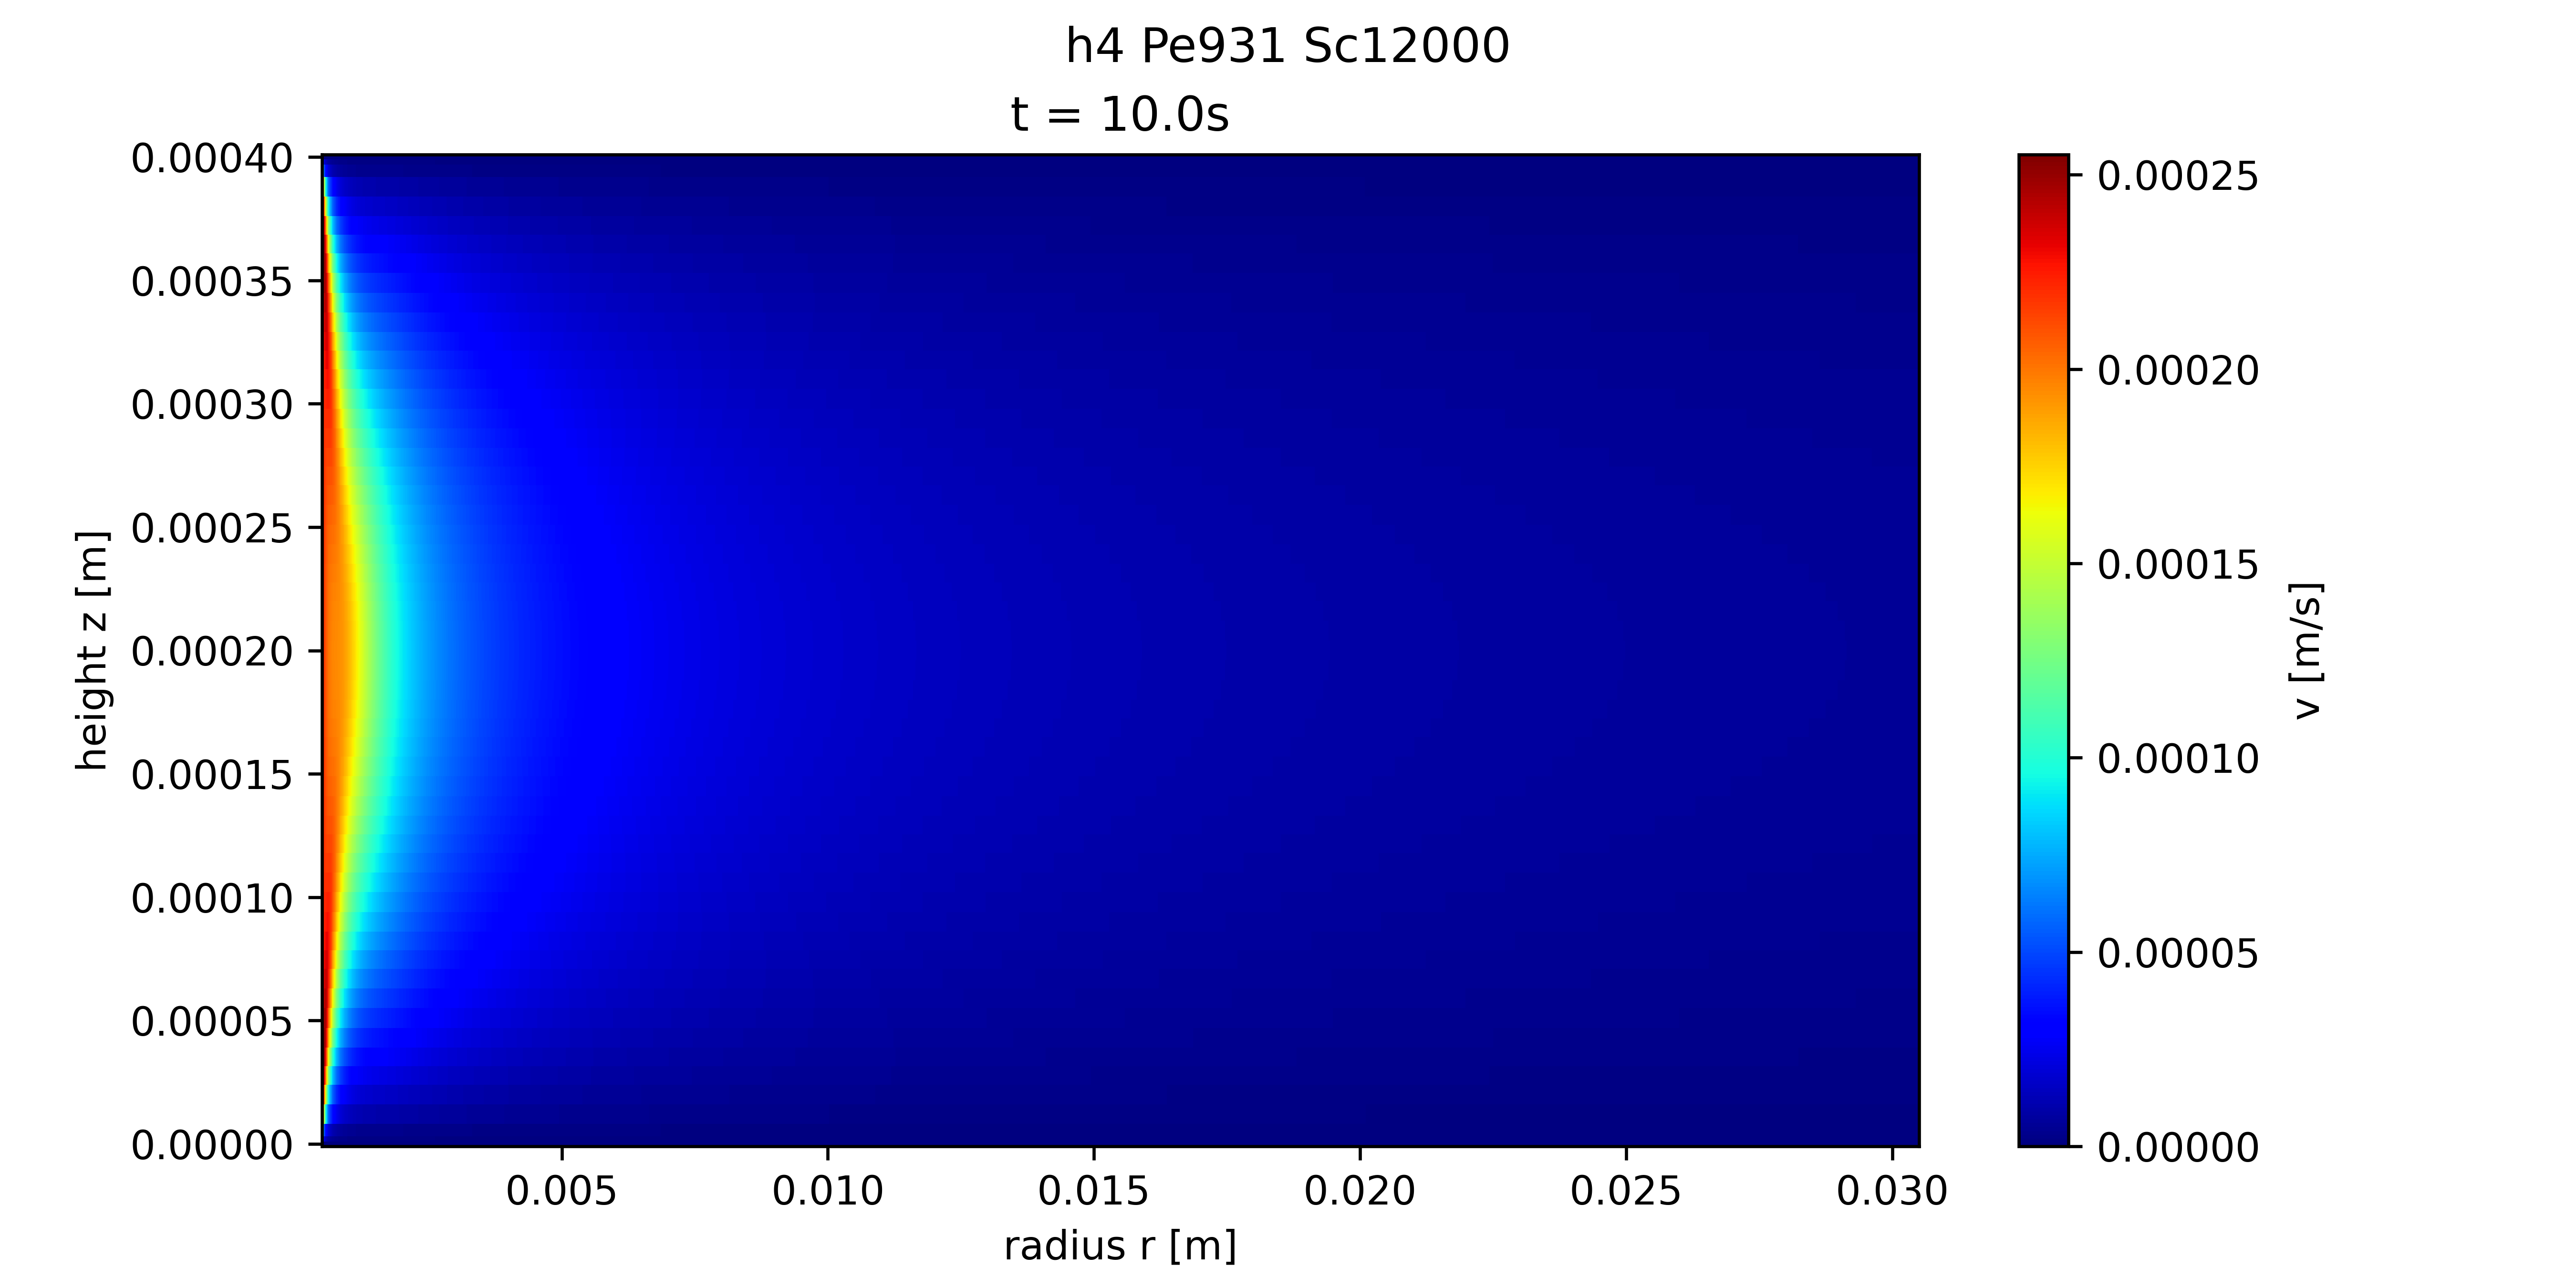
\includegraphics[width=\textwidth]{field_example}
	\caption{example field representation (velocity field) of model results}
	\label{fig: field_example}
\end{figure}
These can be created for all exported variables. Within the example shown the field is created for the velocity magnitude but the variable of most interest is the product concentration. A field example for this variable is shown in \autoref{fig: c_plot_prod_example} for 3 different time steps.
\begin{figure}[htb]
	\centering
	\subfloat[\centering gap averaged concentrations]{{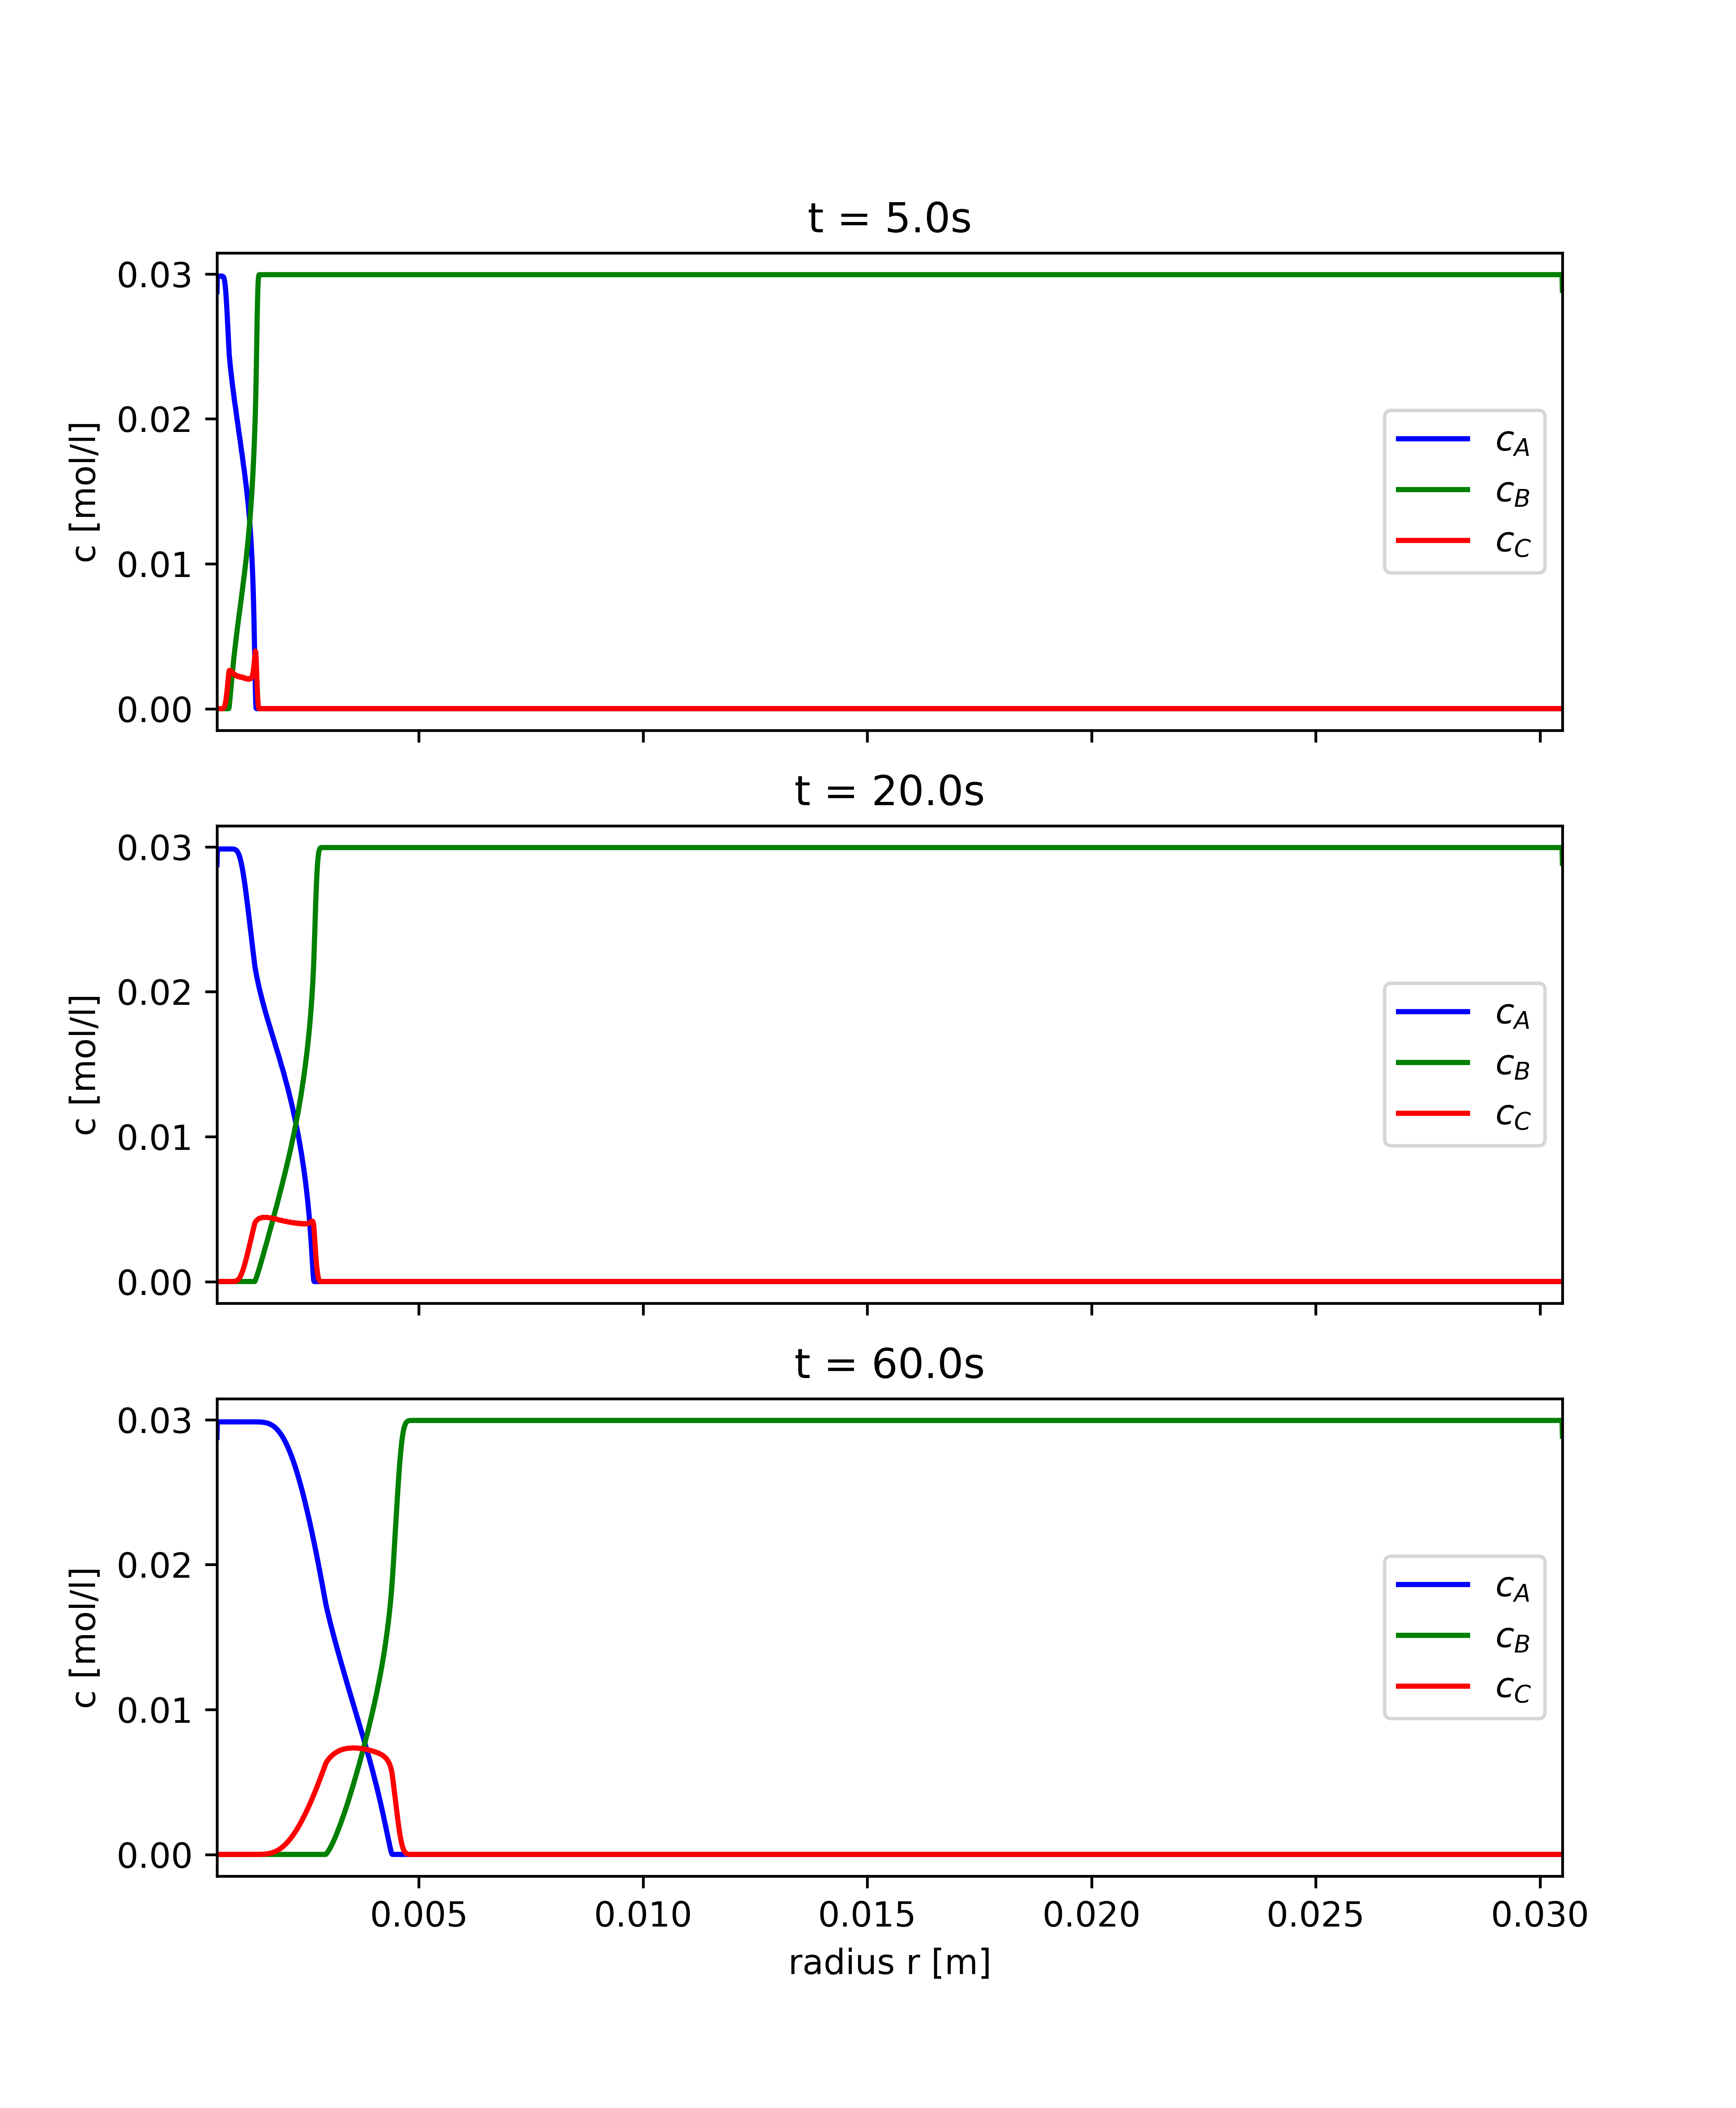
\includegraphics[angle=0, scale=0.41]{plot_h4r3_P931E2_S120E4_concentration-fluid_a_concentration-fluid_b_concentration-fluid_c} }}%
	\qquad
	\subfloat[\centering product concentration fields]{{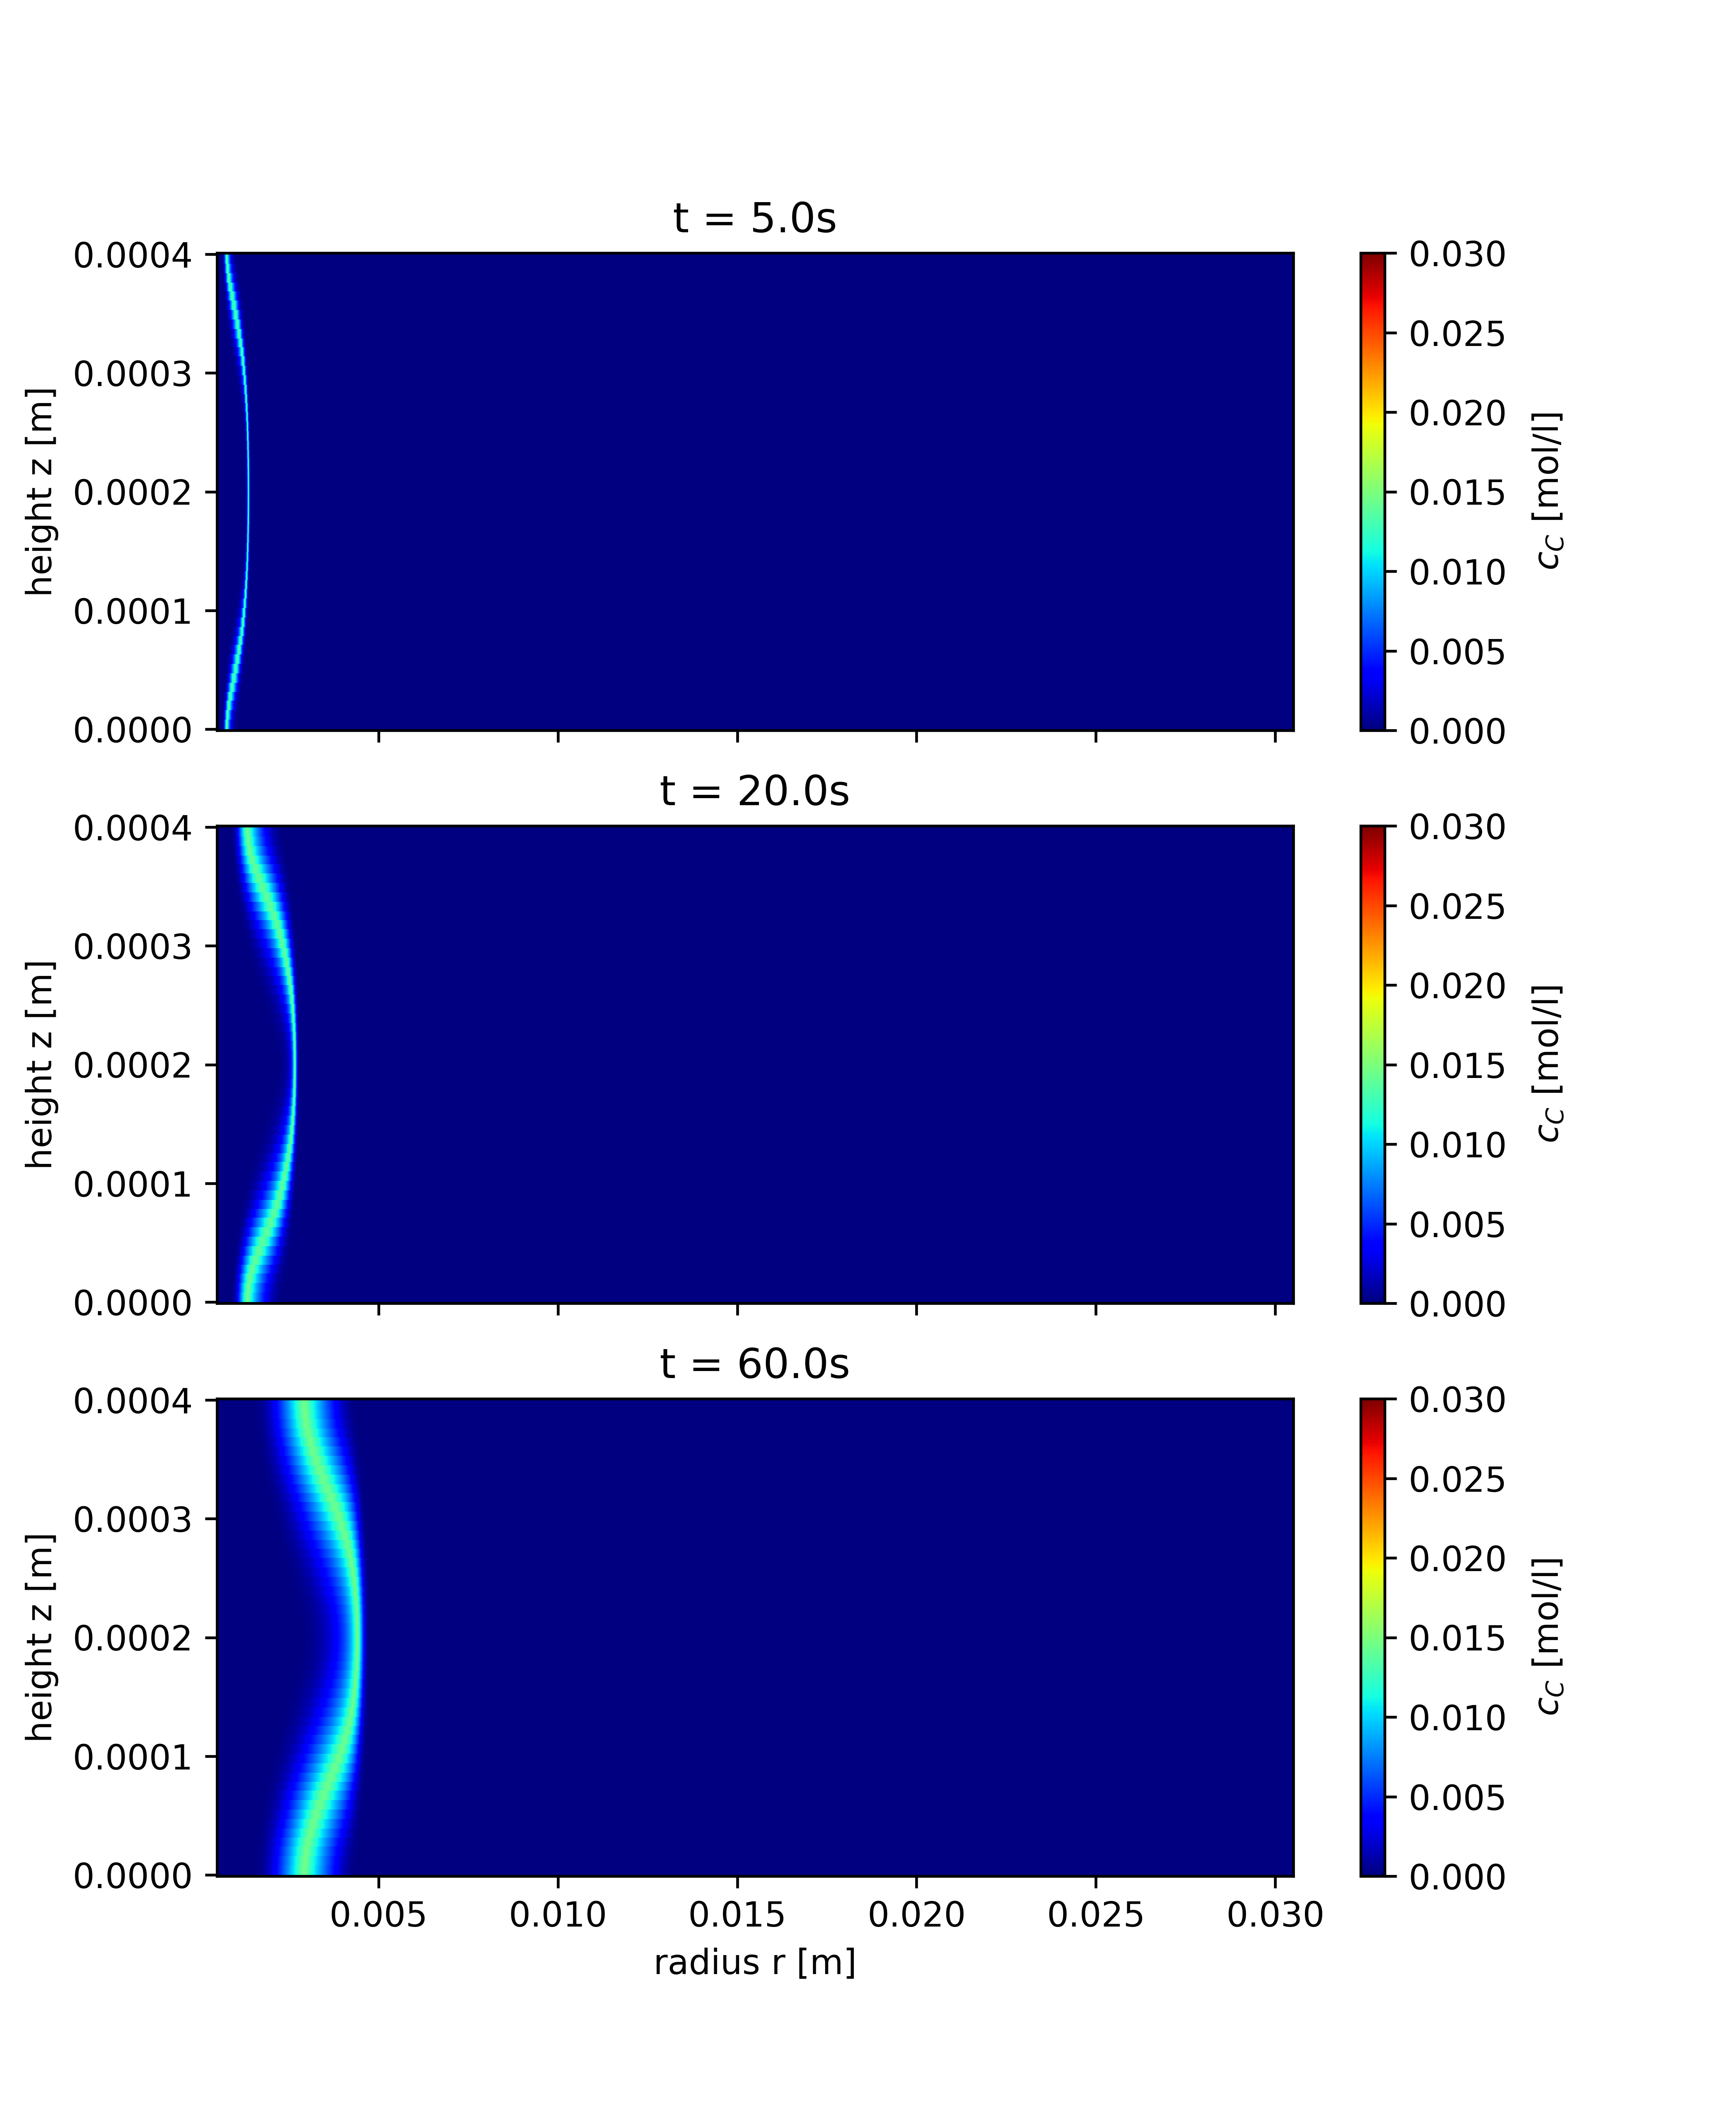
\includegraphics[angle=0, scale=0.41]{field_h4r3_P931E2_S120E4_concentration-fluid_c} }}%
	\caption{field and averaged concentration example}%
	\label{fig: c_plot_prod_example}%
\end{figure}
With these fields the product's concentration can be averaged over the hole gap height. This step is done to get a comparable post-processing step to the image processing done on the experimental data sets. The resulting plots from the previous example can be seen in the same figure as the field example.

With the fields and the gap averaged concentration values computed the parameters of interest can be calculated which is explained within the following sections.

\subsubsection{front positions}

The front's maximum position is gained by storing the radial positions of the product's maxima within the concentration plots. The front's front position is calculated by using the the position furthest away from the center at half the maximums value. The positions gained are shown for one time step in \autoref{fig: pos_examp} as an example.

\begin{figure}[htb]
	\centering
	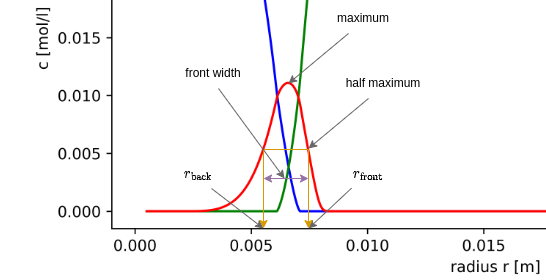
\includegraphics[scale=0.5]{positions_examp}
	\caption{front position procedure schematic}
	\label{fig: pos_examp}
\end{figure}

\subsubsection{front width}

For calculating the front widths the fronts front and back positions are needed. The front position is already gained and the back position is computed using the same approach. Instead of taking for furthest position away from the center the closest one to the inlet is taken to get the back position. The difference between these two radial positions is the front's width at the time. The width calculated is visualized in \autoref{fig: pos_examp}. The approach for calculating the width is also known as \textbf{F}ull \textbf{W}idth at \textbf{H}alf \textbf{M}aximum or FWHM in short.

To gain some more insights a second width is computed. The second width is calculated at the middle of the gap height using the same procedure. Instead of taking the gap averaged values, the values used here are the field values themselves at half the gap height.

\subsubsection{product formed}

Since the cell volume and the product concentration for each cell are exported the total amount of product formed can be calculated ba multiplying these two columns with each other. \texttt{ANSYS FLUENT} computes it's values for one radiant for a 2D case. To gain the amount of product within the hole reactor the values have to be multiplied by $2 \pi$. This procedure can be described by \autoref{eqn: tot_prod}. $ n_{C, total} $ is the total amount of product produced, $n_{cells}$ is the amount of cells in the mesh, $ V_i $ is the volume of one cell and $c_{i, C}$ the product's concentration within that cell $i$.

\begin{equation}
	n_{C, total} = 2 \pi \cdot \sum_{i=0}^{n_{cells}} \left[ V_i \cdot c_{i, C} \right]
	\label{eqn: tot_prod} 
\end{equation}

\subsection{comparison}

For comparison the position of the product's maximum is used. It can be seen that the model and experiment perform similar over hole time range with a small deviation at the early time steps. These difference might come from slightly different flow condition or some mixing due to gravitational influence. Further reasons and possible explanations for the differences within model and experimental results are discussed within \autoref{chp:err_lims}.

\begin{figure}[htbp]
	\centering
	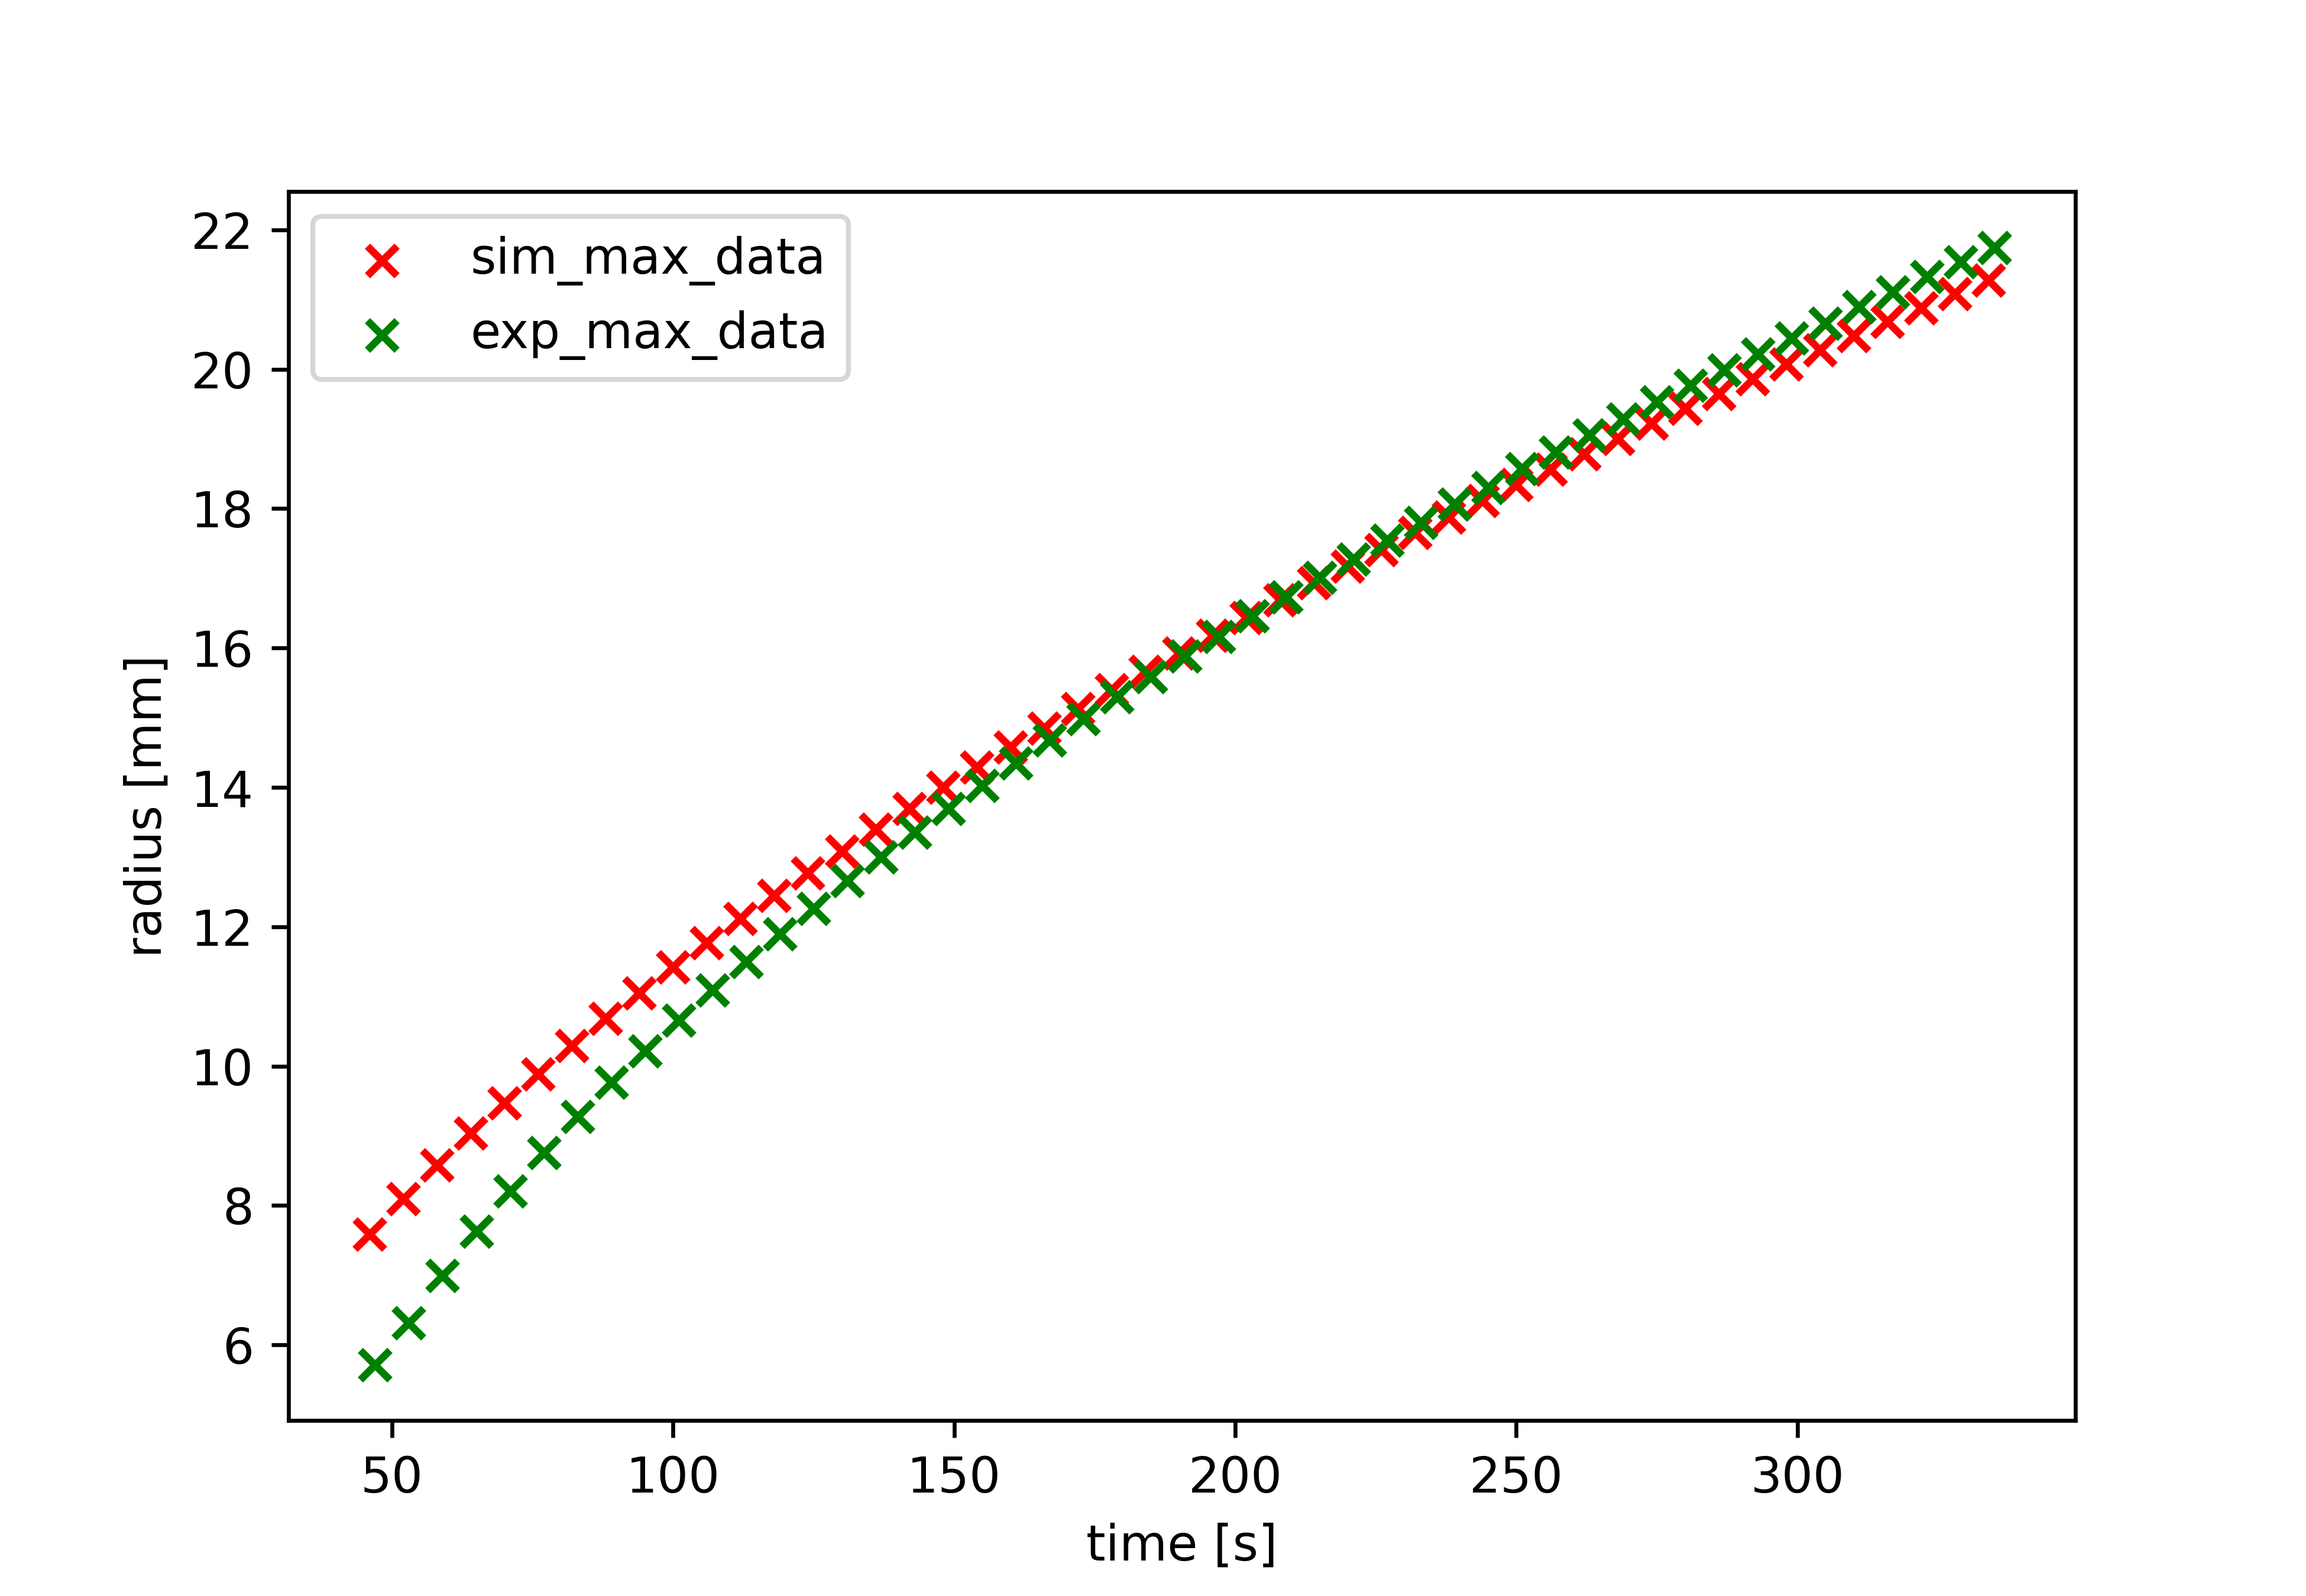
\includegraphics[width=\textwidth]{front_exp}
	\caption{comparison of the experimental and model maxima positions}
	\label{fig: comp_maxis}
\end{figure}
    

\end{document}